%%%%%%%%%%%%%%%%%%%%%%%%%%%%%%%%%%%%%%%%%%%%%%%%%
%------ LaTeX-Template für Abschlussarbeiten, Prof. Thomas Görne, Dezember 2012 --------
%%%%%%%%%%%%%%%%%%%%%%%%%%%%%%%%%%%%%%%%%%%%%%%%%

%---- Header (mit Formateinstellugen) laden, Inputencoding prüfen ------

%%%%%%%%%%%%%%%%%%%%%%%%%%%%%%%%%%%%%%%%%%%%%%%%%
%---- LaTeX-Header fuer Abschlussarbeiten, Prof. Thomas Goerne, Dez. 2012/Aug. 2013 ----
%%%%%%%%%%%%%%%%%%%%%%%%%%%%%%%%%%%%%%%%%%%%%%%%%

\documentclass[12pt,paper=A4,pointlessnumbers,bibtotoc,liststotoc,DIV=11,BCOR=1mm]{scrreprt}
% BCOR ist die Bindekorrektur (verlorener Rand am linken Blattrand)! Wert haengt von der Art der Heftung ab!!
% DIV ist eine Satzspiegeleinstellung von KOMA-Script / sccreprt.

\pagestyle{headings}

\usepackage[T1]{fontenc} % Font Encoding fuer europaeische Schriften mit Umlauten (Unterstuetzung der Worttrennung)
\usepackage{lmodern} % PostScript-Varianten der TeX Computer Modern-Schriften laden
\usepackage[english,ngerman]{babel} % Spracheinstellungen fuer Englisch und Neudeutsch laden

\usepackage{graphicx} % Grafikeinbindung (fuer .JPG, .JPEG, .PNG und .PDF, falls pdflatex benutzt wird)
\usepackage[table]{xcolor} % ermoeglicht farbige Schrift und farbige Tabellenzeilen
\definecolor{black}{gray}{0} % Umdefinition der Farbe black, falls noetig (0=schwarz, 1=weiss)
\definecolor{dblue}{rgb}{0.1,0.2,0.6} % Dunkelblau, fuer Hyperlinks
\definecolor{lgray}{gray}{0.9} % Hellgrau, fuer Tabellen (0=schwarz, 1=weiss)

\usepackage{booktabs} % fuer schoene Tabellen

\usepackage[round,authoryear]{natbib} % Literaturverweise mit Name/Jahreszahl in runden Klammern
\bibpunct[:\,]{(}{)}{,}{a}{}{,~}  % Feinformatierung der Natbib-Zitierweise

\usepackage[hyphens]{url}
\usepackage[colorlinks=true,linkcolor=black,citecolor=dblue,urlcolor=dblue]{hyperref} 
\usepackage{hyperref}  
% die Pakete url und hyperref ermoeglichen anklickbare URLs im Quellenverzeichnis in definierter Farbe, 
% sie ermoeglichen den Zeilenumbruch bei langen URLs, und sie erzeugen Hyperlinks (Farbe s.o.) 
% zwischen Quellenverweis und Quellenverzeichnis sowie zwischen label und ref im PDF-Dokument

% Fonteinstellungen fuer Bildunterschriften: Unterschrift serifenlos, "Abbildung" fett (bfseries = bold face series)
\setkomafont{captionlabel}{\sffamily\bfseries}
\setkomafont{caption}{\sffamily}

%------------------------------------------------------------------------------------------------------------------
%------ Eigenstaendigkeitserklaerung im gerahmten Kasten (parbox in einer framebox) ------
%------------------------------------------------------------------------------------------------------------------

\newcommand{\eigen}{
\setlength{\fboxsep}{2ex}
\setlength{\fboxrule}{0.8pt} 
% Einstellungen fuer Rahmenabstand und Rahmendicke der Framebox
\begin{center}
	\fbox{
		\parbox{0.8\linewidth}{
		Ich versichere, die vorliegende Arbeit selbstst\"andig ohne fremde Hilfe verfasst 
		und keine anderen Quellen und Hilfsmittel als die angegebenen benutzt zu haben. 
		Die aus anderen Werken w\"ortlich entnommenen Stellen oder dem Sinn nach 
		entlehnten Passagen sind durch Quellenangaben eindeutig kenntlich gemacht.
		\par\bigskip\bigskip\bigskip\bigskip
		\hspace*{0.8cm}Ort, Datum \hfill \vorname~\nachname\hspace*{0.8cm}
		}
	}
\end{center}
}

%%%%%%%%%%%%%%%%%%%%%%%%%%%%%%%%%%%%%%%%%%%%%%%%%


%------------------------ Titelblatt-Layout laden ----------------------------------

%%%%%%%%%%%%%%%%%%%%%%%%%%%%%%%%%%%%%%%%%%%%%%%%%
%------ LaTeX-Titelblatt fuer Bachelorarbeiten, Prof. Thomas Goerne, Dezember 2012 -------
%------------------------------------------------------------------------------------------------------------------
%--------------------------------- Deklarationen fuer die Titelseite  --------------------------------------
%%%%%%%%%%%%%%%%%%%%%%%%%%%%%%%%%%%%%%%%%%%%%%%%%

\title{\titel\\[2ex]
\LARGE Bachelor-Thesis\\
\large zur Erlangung des akademischen Grades B.Sc.\\[1.5ex]
\LARGE \vorname~\nachname\\[0.5ex] 
\large \matrikelnummer
}

\author{\unitlength1mm
\large\raisebox{-1ex}{
\includegraphics[width=4em]{HAW_wuerfel}}\hspace{1ex}
\parbox[b]{11.2cm}{\sffamily\large%
Hochschule f\"ur Angewandte Wissenschaften Hamburg\\[-0.2ex]
Fakult\"at Design, Medien und Information\\[-0.2ex]
Department Medientechnik
}\\[6ex]
\sffamily\large Erstpr\"ufer: \erstpruef\\[0.5ex]
\sffamily\large Zweitpr\"ufer: \zweitpruef}

%%%%%%%%%%%%%%%%%%%%%%%%%%%%%%%%%%%%%%%%%%%%%%%%%
%\input{hawmt-master-titelblatt}

%---------------------------- Titeldefinitionen --------------------------------------

\newcommand{\vorname}{Matthias}
\newcommand{\nachname}{Held}
\newcommand{\matrikelnummer}{2182712}

\newcommand{\titel}{\glqq Red Tail\grqq\ :\\ Auswirkung eines zusätzlichen tiefroten Spektralanteils auf das Weißlicht von LED-Scheinwerfern\\[0.2ex] 
				\Large - am Beispiel der Beleuchtung von Hauttönen im TV-Bereich}

\newcommand{\erstpruef}{Prof. Dr. Roland Greule}
\newcommand{\zweitpruef}{Dipl. Ing. (FH) Matthias Allhoff}

\date{vorläufige Fassung vom \today}   % praktisch für Vorab-Versionen. 
%\date{\sffamily Hamburg, 2. 2. 2020}  % Abgabedatum!

%--------------------------------------------------------------------------------------
%----------------------------- hier gehts los! --------------------------------------
%--------------------------------------------------------------------------------------

\begin{document}
\selectlanguage{ngerman}
\maketitle           % Titelseite erzeugen
\tableofcontents % Inhaltsverzeichnis erzeugen
\clearpage          % Seitenumbruch


%------------ Zusammenfassung / Abstract ------------------

\thispagestyle{empty}
\selectlanguage{english}
\section*{\centering\abstractname}
Form and layout of this \LaTeX-template incorporate the guidelines for theses in the Media Technology Department \glqq Richtlinien zur Erstellung schriftlicher Arbeiten, vorrangig Bachelor-Thesis (BA) und Master-Thesis (MA) im Department Medientechnik in der Fa\-kul\-t{\"a}t DMI an der HAW Hamburg\grqq\ in the version of December 6, 2012 by Prof.\ Wolfgang Willaschek. 

The thesis should be printed single-sided (simplex). The binding correction (loss at the left aper edge due to binding) might be adjusted, according to the type of binding. This template incorporates a binding correction as BCOR=1mm (suitable for adhesive binding) in the \LaTeX\ document header.

{\bfseries This is the english version of the opening abstract} (don't forget to set \LaTeX's language setting back to ngerman after the english text). 
 
 
\selectlanguage{ngerman}
\section*{\centering\abstractname}

Diese Arbeit befasst sich mit der Auswirkung eines zusätzlichen tiefroten Spektralanteils auf das kaltweiße Lichtspektrum von LED-Scheinwerfern. Es soll dabei überprüft werden, ob Personen unter diesen Umständen im Kamerabild natürlicher aussehen, wie es in der \glqq Red Tail\grqq\ - Theorie der mo2 design GmbH angenommen wird.\\
Zunächst wird auf wichtige Kenngrößen der Lichttechnik eingegangen und verschiedene Leuchtmittel und lichttechnische Parameter werden erläutert. Im Folgeneden werden die Messungen beschrieben.\\
Bei diesen wird ein LED-Scheinwerfer und ein rotgefilterter PAR-Scheinwerfer, der den\glqq Red Tail\grqq\ simulieren soll, auf einen Messpunkt ausgerichtet. Der LED-Scheinwerfer wird zuerst allein auf eine kaltweiße Referenzlichtquelle bestmöglich abgeglichen und spektral vermessen. Anschließend wird der rotgefilterter PAR-Scheinwerfer dazugeschlatet und auch dieses Lichtgemisch wird auf die Referenzlichtquelle abgeglichen und spektral vermessen. 
Bei der Auswertung werden die gemessenen lichttechnischen Parameter betrachtet und zusätzlich werden bei einer Umfrage Bilder verglichen, auf denen Probanden verschiedener Hauttöne mit und ohne \glqq Red Tail\grqq\ beleuchtet wurden.




%--------------------------- Text -------------------------------

\chapter{Einleitung}

\chapter{Grundlagen und Kenngrößen der Lichttechnik} \label{chap_grundlagen}

\section{Lichtstrom $\Phi$} \label{sec_lumen}

\section{Beleuchtungsstärke E}\label{sec_lux}

\section{Lichtstärke I}\label{sec_candela}

\section{Leuchtdichte L}\label{sec_candelamm}

\chapter{Farbe und Farbräume}
In diesem Kapitel wird auf die Grundlagen der Farben und Farbräume eingegangen.
%Einleitung vernünftig schreiben

\section{Farben mit dem Auge sehen} \label{sec_auge}
% Einleitender Satz fehlt

Es gibt zwei verschiedene Fälle, in denen der Mensch die Gesichtsemfpindung Farbe verspürt: Entweder leuchtet ein Objekt von selbst, sodass dessen Licht aus einem Spektralbereich des sichtbaren Spektrums ins Auge gelangt und dann im Zusammenspiel mit dem Gehirn ein Farbreiz $\phi(\lambda)$ erzeugt. In diesem Fall nennt man das Objekt einen Selbstleuchter. Die zweite Möglichkeit ist, dass das Objekt von einer Lichtquelle beleuchtet wird und das reflektierte Lichtspektrum wahrgenommen wird. Der Gegenstand aborbiert und transmittiert bestimme spektrale Anteile des Lichts und reflektiert den für den Farbton verantworlichen Rest (Kapitel \ref{chap_grundlagen}). Daher erscheint beispielsweise ein roter Apfel von blauem Licht beleuchtet unbunt, da kein roter Spektralanteil im blauen Licht vorhanden ist.
In diesem zweiten Fall spricht man von Körperfarben\footnote{\cite[103]{hentschel}}.\\     
Damit ein Mensch so einen Farbreiz wahrnehmen kann, gibt es im Auge zwei Arten von lichtempfindlichen Rezeptoren in der Netzhaut, die für unsere Farbwahrnehmung verantwortlich sind: Zapfen und Stäbchen.\\
Die Stäbchen nehmen verschiedene Helligkeitseindrücke wahr, können aber keine Farben unterscheiden. Daher sind sie für das skotopische Sehen (Nachtsehen) von $3 \cdot 10^{-6} \frac{cd}{m^{2}}$ bis 0,03$\frac{cd}{m^{2}}$ verantwortlich \footnote{\cite{doccheck sko}}.
Die verschiedenen spektralen Anteile des Lichts wirken sich auf die Zapfen aus und verantworten so den Farbeindruck. Außerdem sind die Zapfen für das photopische Sehen (Tagessehen), ab einer Leuchtdichte von 3$\frac{cd}{m^{2}}$, zuständig \footnote{\cite{doccheck pho}}.\\
Der Mensch kann Wellenlängen von 380nm bis 780nm wahrnehmen. Jedoch ist das Auge nicht für alle Farben gleich empfindlich. Grüne Gegenstände (555nm) wirken immer heller als blaue (485nm) oder rote (680nm). Dieser Sachverhalt wurde mit der V($\lambda$)-Kurve  aufgezeigt (Abbildung \ref{b_augespek}).
 

\begin{figure}[H]     % h=here, t=top, b=bottom, p=page
\centering
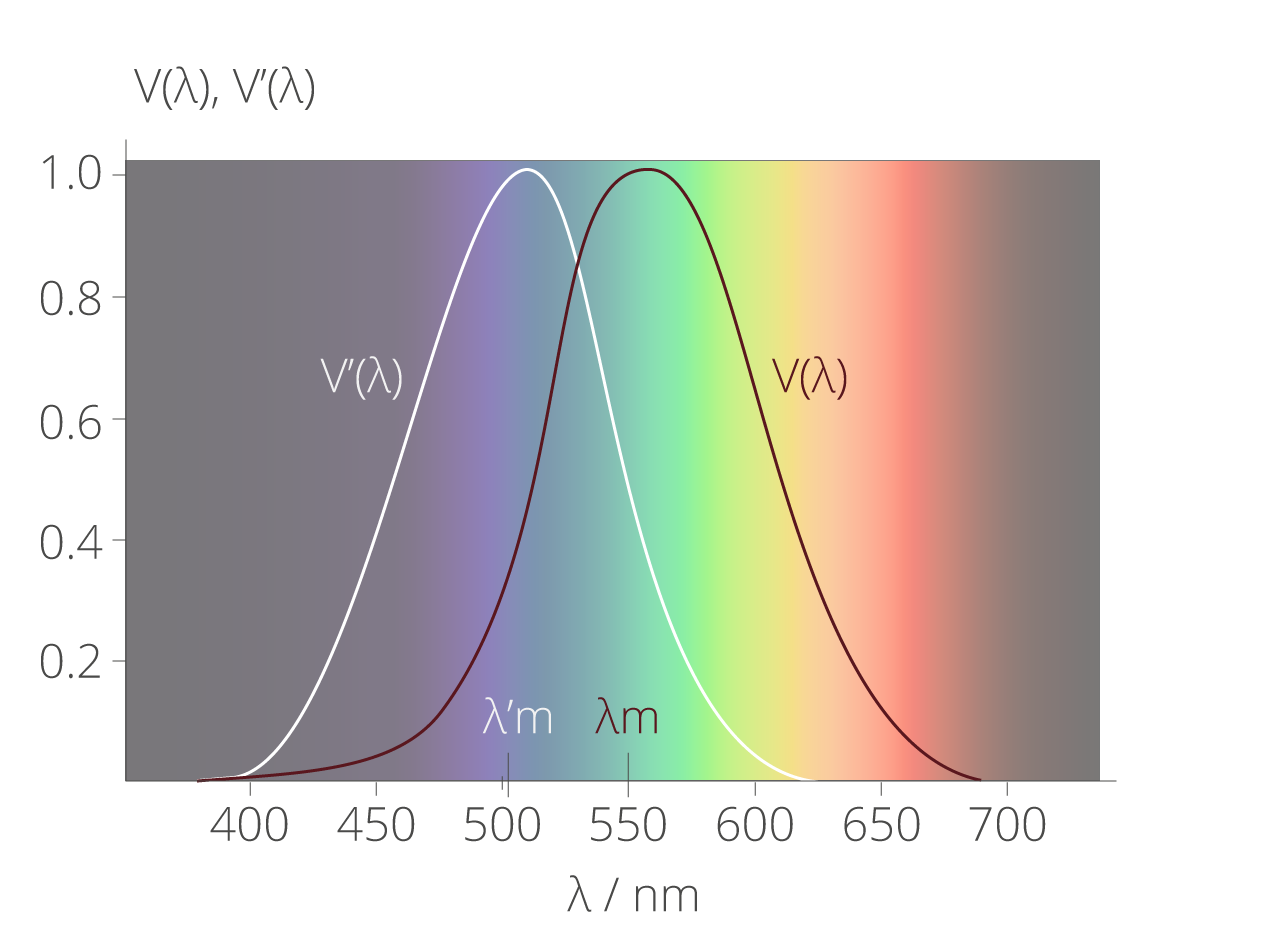
\includegraphics[width=0.7\textwidth]{bilder/augespek} 
% Bilddatei aus dem Unterverzeichnis bilder holen, skalieren auf 0.8*Satzspiegel
\caption {Die V($\lambda$)-Kurve zeigt, wie das Auge die verschiedenen Wellenlänge beim photopischen Sehen gewichtet. Die weiße Kurve (V'($\lambda$)) beschreibt, wie sich das Farbsehen beim Nachtsehen verschiebt. \protect\footnotemark}\label{b_augespek}
\end{figure}

\footnotetext{\url{https://www.gigahertz-optik.de/assets/Uploads/Abb.-II.13-neu-v03.png}}


Mit den Zapfen und Stäbchen kann ein Mensch bis zu 200 verschiedene Farbtöne wahrnehmen. Wenn man die verschiedenen möglichen Helligkeiten und Weißkombinationen dieser Farbtöne zusätzlich in Betracht zieht, kann man von ca. 20 Millionen unterschiedlichen Farben sprechen, die ein Mensch erkennen kann \footnote{\cite{unimann}}.
 
Um all diese Farben unterscheiden zu können gibt es nach Young und Helmholtz drei Rezeptortypen. Die \glqq Trichromatische Theorie\grqq besagt, dass es grüne, blaue und rote Zapfen gibt, die unterschiedlich empfindlich für die jeweiligen Spektralanteile des Lichtes sind. Aus diesen drei Farbinformation (RGB-Werte) entsteht dann im Gehirn eine Farbe. Auf diese Weise lassen sich aber nicht alle Phänomene der Farbwahrnehmung erklären. 1878 hat Hering eine andere Theorie entwickelt, wie Farben wahrgenommen werden und diese \glqq Gegenfarbentheorie\grqq genannt. Die Theorie besagt, dass es immer zwei Farben gibt, die sich gegensätzlich verhalten: rot und grün, blau und gelb und der unbunte Gegensatz schwarz (dunkel) und weiß (hell).\\ Nach ein paar Jahren der Uneinigkeit, welche der genannten Theorie denn nun korrekt ist, hat 1905 v. Kries mit seiner \glqq Zonentheorie\grqq herausgestellt, dass beide Theorien zugleich zutreffen. Einerseits wird im Auge nach der \glqq Trichromatische Theorie\grqq eine Farbe als RGB-Stimulus wahrgenommen, dieser wird dann andererseits nach der \glqq Gegenfarbentheorie\grqq im Gehirn mit den drei Farbgegensätzen ausgewertet \footnote{\cite[104]{hentschel}} (Abbildung \ref{b_zonen}).

 
\begin{figure}[H]     % h=here, t=top, b=bottom, p=page
\centering
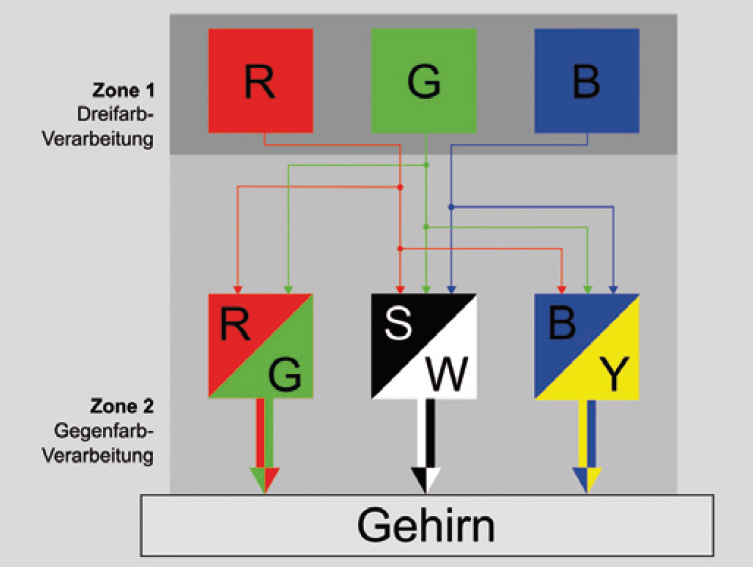
\includegraphics[width=0.7\textwidth]{bilder/zonen} 
% Bilddatei aus dem Unterverzeichnis bilder holen, skalieren auf 0.8*Satzspiegel
\caption {Darstellung der Zonentheorie von v. Kries \protect\footnotemark}\label{b_zonen}
\end{figure}
\footnotetext{\cite[153]{greule}}

% Überleitung einfügen

Bei der additiven Farbmischung werden die Spektralanteile verschiedener Farbtöne als Mischfarbe erkannt. Dies kann auf unterschiedliche Weisen passieren. Entweder treffen zwei verschiedene Spektralanteile auf den gleichen Punkt auf der Netzhaut und lösen so einen Farbreiz aus. Oder das Licht verschiedener Wellenlängen trifft auf unterschiedliche Teile der Netzhaut, die so dicht aneinander sind, dass das Auge daraus eine Farbe mischt (örtliche Nähe). Oder derselbe Punkt auf der Netzhaut wird von zwei verschiedenen Spektralanteilen mit einer Wechselfrequenz von $f\geq25Hz$ getroffen (zeitliche Nähe). Oder das Licht verschiedener Wellenlängen trifft auf unterschiedliche Teile der Netzhaut, die so dicht aneinander sind, dass das Auge daraus eine Farbe mischt.\\
Grundsätzlich werden bei jeder Art der additiven Farbmischung die Strahlungsleistungen der Spektralanteile $\Phi_{e\lambda,i}(\lambda)$ zusammenaddiert\footnote{\cite[83]{greule}}(Gleichung\ref{gl_farbe+}).

	\begin{equation}\label{gl_farbe+}
		\Phi_{e\lambda}(\lambda) = \Phi_{e\lambda,1}(\lambda) + \Phi_{e\lambda,2}(\lambda) + \Phi_{e\lambda,3}(\lambda)
	\end{equation}\\


1853 hat Grassmann zur additiven Farbmischung drei allgemein gültige Regeln aufgestellt \footnote{\cite[105]{hentschel}}: 
\newpage
\begin{enumerate}\setlength{\itemsep}{0ex}
\item Für das Ergebnis einer additiven Farbmischung ist nur das Aussehen, nicht die spektrale Zusammensetzung der Komponenten maßgebend.
\item Alle Farbmischungen verlaufen stetig.
\item Zum Festlegen einer Farbe sind drei Bestimmungsstücke notwendig und hinreichend.
\end{enumerate}

Die erste Regel beschreibt beispielweise das Verhalten einer Tomate unter gemischtem und ungemischtem magentafarbenen Licht. Wird die Tomate von einem magentanen Licht bestrahlt, dessen Spektrum nur Anteile im Magentabereich hat, so wird die Tomate weitesgehend unbunt erscheinen, weil diese alle spektralen Anteile des Lichts, außer den roten, absorbiert. Falls man aber rotes Licht mit blauem Licht mischt und so die selbe Lichtfarbe wie von dem reinen magentafarbigen Licht erzeugt, so erscheint die Tomate unter diesem Licht wiederum trotzdem rot, da die Rot-Anteile im Spektrum vorhanden sind. Man kann jedoch mit dem bloßen Auge diese beiden Farben nicht unterscheiden (metamere Farben), da der Mensch die spektrale Zusammensetzung von Licht nicht wahrnimmt. 

Die zweite Regel zeigt auf, dass bei der additiven Farbmischung die Farben stets ineinander übergehen und kein Sprung dabei entsteht, wenn zwei Farben zu einer Mischfarbe werden.

Die dritte Regel besagt, dass Farben beispielsweise mit Helligkeit, Farbton und Sättigung ausreichend beschrieben sind, um sie eindeutig zu definieren und reproduzieren zu können. Auch mit den Farbanteilen von den Grundfarben Rot, Blau und Grün können Farben definiert werden (Kapitel \ref{b_farben+}).   

\begin{figure}[H]     % h=here, t=top, b=bottom, p=page
\centering
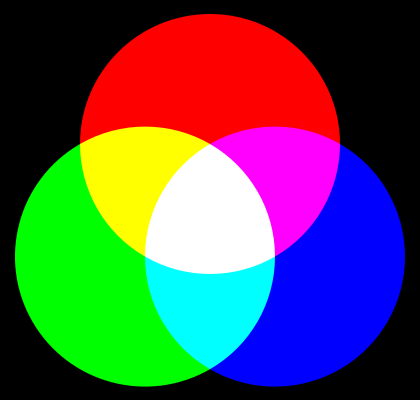
\includegraphics[width=0.5\textwidth]{bilder/farben+} 
% Bilddatei aus dem Unterverzeichnis bilder holen, skalieren auf 0.8*Satzspiegel
\caption {Die drei Grundfarben Rot, Grün und Blau der additiven Farbmischung ergeben zusammen weiß (unbunt).\protect\footnotemark}\label{b_farben+}
\end{figure}

\footnotetext{\url{https://upload.wikimedia.org/wikipedia/commons/thumb/e/e0/Synthese\%2B.svg/420px-Synthese\%2B.svg.png}}

Bei der subtraktiven Farbmischung geht es nicht um die Farbwahrnehmung des Auges, sondern um Licht im rein physikalischen Sinne. Ein subtraktives Farbgemisch entsteht, wenn die Transmissions- und Reflektionseigenschaften zweier Farben miteinander multipliziert werden\footnote{\cite[84]{greule}} (Gleichung \ref{gl_farbe-}).

\begin{equation}\label{gl_farbe-}
		T(\lambda) = T_{1}(\lambda) \cdot T_{2}(\lambda) \cdot T_{3}(\lambda)
	\end{equation}
Die Formel stellt ein Beispiel für das Produkt der Transmissionswerte dar.
Hierbei handelt es sich um ein wesentlich komplizierteren Prozess, als bei der additiven Farbmischung. Da durch diese Multiplikation der Farben ein spektraler Anteil entfällt, spricht man von einer subtraktiven Farbmischung, obwohl das Produkt der Farbeigenschaften gebildet wird (Abbildung \ref{b_farben-}).

\begin{figure}[H]     % h=here, t=top, b=bottom, p=page
\centering
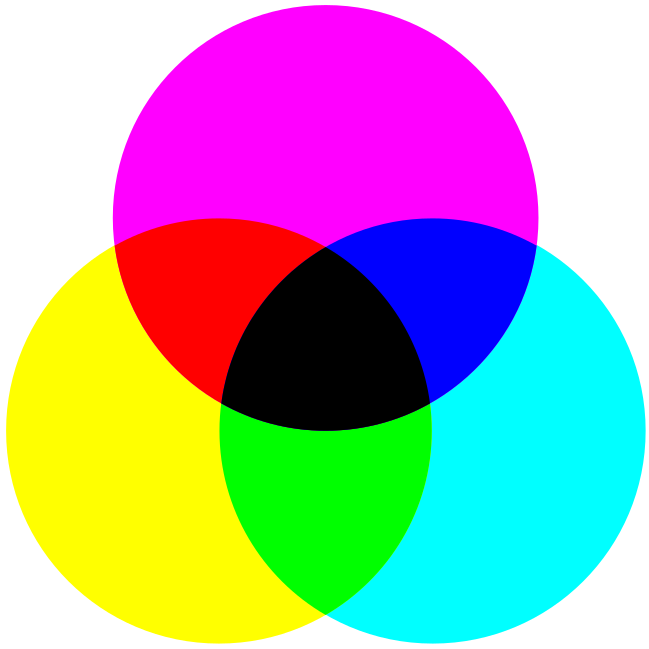
\includegraphics[width=0.5\textwidth]{bilder/farben-} 
% Bilddatei aus dem Unterverzeichnis bilder holen, skalieren auf 0.8*Satzspiegel
\caption {Die drei Grundfarben Cyan, Magenta und Gelb der subtraktiven Farbmischung ergeben zusammen schwarz (unbunt).\protect\footnotemark}\label{b_farben-}
\end{figure}

\footnotetext{\url{https://upload.wikimedia.org/wikipedia/commons/thumb/6/64/CMY_ideal_version_rotated.svg/649px-CMY_ideal_version_rotated.svg.png}}

%Überleitung zum RGB Farbraum


 
\section{RGB Farbraum} \label{sec_rgb}

\section{CIE-XYZ Farbraum} \label{sec_xyz}

\section{CIE-LUV Farbraum} \label{sec_luv}

\section{CIE-LAB Farbraum} \label{sec_lab}

\chapter{Lichtechnische Parameter}
Es gibt mehr als vierzig verschiedene Methoden, um die Farbwiedergabe einer Leuchte zu beurteilen. In diesem Kapitel sollen die in der Medien- und TV-Branche typischen Farbwiedergabeindices vorgestellt und deren Relevanz für die Messung mit dem \glqq Red Tail\grqq  aufgezeigt werden.

\section{CIE: Color Rendering Index (CRI)} \label{sec_cri}

Da der Farbort allein keine eindeutige Aussage über die Zusammensetzung des Spektrums zulässt, wurde 1965 von der Commission Internationale de l'Eclairage ein Testverfahren entwickelt, mit dem man die Farbwiedergabe (Color Rendering Index) einer Leuchte bestimmen kann. Dafür hat man acht Referenzfarben festgelegt. Bei einer CRI-Messung überprüft man also, wie gut eine Lichtquelle diese Körperfarben wiedergeben kann. Es wird dabei zwischen einem schwarzen Strahler(< 5000K) und Tageslicht(> 5000K) differenziert. Die gemessenen Unterschiede zu den Referenzfarben werden mit Werten von 0 bis 100 gewichtet($R_{1}$-$R_{8}$), wobei ein Wert von 100 aussagt, dass die Farbe bestmöglich wiedergegeben wird. Zuerst werden die einzelnen Indexwerte $R_{i}$ aus den Farbdifferenzen $\Delta E_{i}$ berechnet (Gleichung \ref{gl_cri1})\footnote{\cite{davis_ohno}}.

	\begin{equation}\label{gl_cri1}
		R_{i} = 100 - 4,6 \cdot \Delta E_{i}
	\end{equation}
Diese acht Werte werden schließlich arithmetisch gemittelt und es ergibt sich der Gesamtwert $R_{a}$ (Gleichung \ref{gl_cri2})\footnote{\cite{production partner}}.
	\begin{equation}\label{gl_cri2}
		R_{a} =\frac{1}{8} \sum_{i=1}^{8} R_{i}
	\end{equation}
In der DIN 6169 werden zur besseren Beurteilung der Farbwiedergabe die $R_{a}$-Werte in verschiedene Stufen unterteilt (Tabelle \ref{t_cri}).

	\begin{table}[htp] 
		\rowcolors{1}{}{lgray} 
		\centering
		\begin{tabular}{rlcc}  % Spalten nach Ausrichtung: l, c, r, p{breite} 
		\toprule
		\multicolumn{3}{c}{\large\sffamily Stufen des CRI}\\ 							
		\midrule
		1A & $R_{a} \geq 90$ & sehr hohe Anforderung\\ 
		1B & 90 > $R_{a} \geq 80$ & sehr hohe Anforderung\\
		2A & 80 > $R_{a} \geq 70$ & hohe Anforderung\\
		2B & 70 > $R_{a} \geq 60$ & hohe Anforderung\\
		3 & 60 > $R_{a} \geq 40$ & mittlere Anforderung\\
		4 & 40 > $R_{a} \geq 20$ & geringe Anforderung\\
		\bottomrule
		\end{tabular}
		\caption{$R_{a}$ eingeteilt in verschiedene Stufen\protect\footnotemark}	
		\label{t_cri}
	\end{table}
	\footnotetext{\cite[111]{hentschel}}

Ein hoher $R_{a}$-Wert beschreibt aber nur bedingt die Farbwiedergabe einer Leuchte, da beispielsweise keine Angabe über die Sättigung der Farben gemacht wird. Außerdem sind die acht Referenzfarben nur Pastelltöne, weil der CRI damals für Glühlicht entwickelt wurde. Gesättigte Farben fließen nicht in die Bewertung mit ein.
Das wirkt sich auch auf die Vergleichbarkeit von Leuchten aus. Zwei Scheinwerfer mit dem selben $R_{a}$-Wert von 90 können sehr unterschiedliche Spektren haben und damit sehr unterschiedlich Farben darstellen, trotz gleichem Farbwiedergabeindex.
Außerdem kann man nur schwer eine Aussage darüber machen, ob sich eine Leuchte mit einem guten CRI für Personenbeleuchtung eignet, weil Rottöne und Hauttöne in diesem Bewertungsverfahren fehlen.\\\\
Leuchtstofflampen nutzten den CRI aus, indem durch gezielte schmalbandige Peaks im Spektrum die Referenzfarben getroffen werden. Auf diese Weise kann zwar ein hoher CRI-Werte erreicht werden, aber kein breitbandiges und ausgefülltes Lichtspektrum entstehen. Daher sah sich die CIE gezwungen den Farbwiedergabeindex zu erweitern. In dem neueren $R_{e}$-Wert gibt es nun auch gesättigte Farben und eine Hautfarbe wird miteinbezogen (Abb. \ref{b_cri}).

\begin{figure}[htp]     % h=here, t=top, b=bottom, p=page
\centering
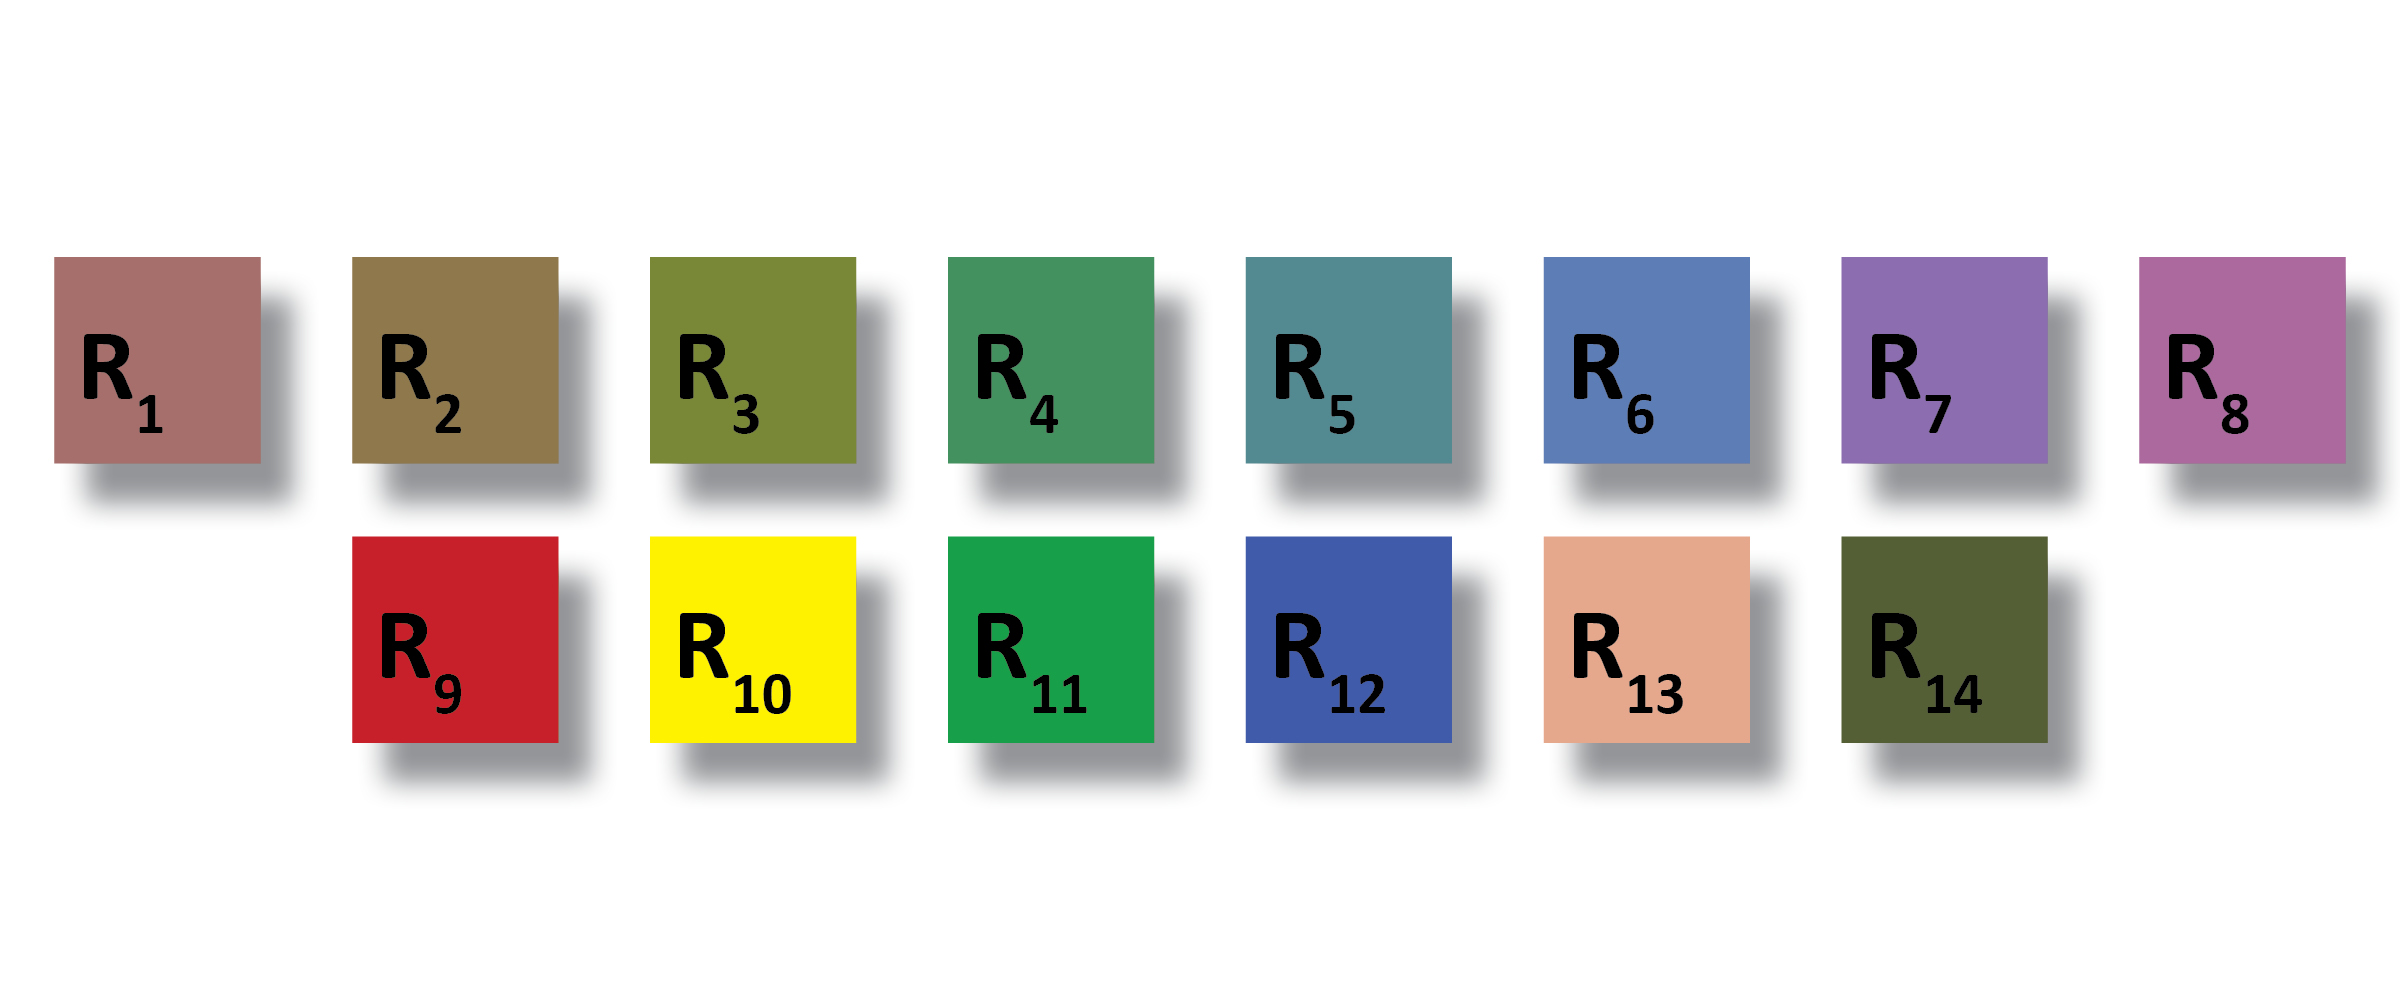
\includegraphics[width=0.8\textwidth]{bilder/cri} 
% Bilddatei aus dem Unterverzeichnis bilder holen, skalieren auf 0.8*Satzspiegel
\caption {Alle Referenzfarben des Farbwiedergabeindexes: $R_{1}$ Altrosa, $R_{2}$ Senfgelb, $R_{3}$ Gelbgrün, $R_{4}$ Hellgrün, $R_{5}$ Türkisblau, $R_{6}$ Himmelblau, $R_{7}$ Asterviolett, $R_{8}$ Fliederviolett, $R_{9}$ Rot gesättigt, $R_{10}$ Gelb gesättigt, $R_{11}$ Grün gesättigt, $R_{12}$ Blau gesättigt und $R_{13}$ Rosa (Hautfarbe), $R_{14}$ Blattgrün \protect\footnotemark}\label{b_cri}
\end{figure}

\footnotetext{\url{https://www.elementalled.com/wp/wp-content/uploads/2015/08/CRI_chart.jpg}}


Bei einer warmweißen LED konnte ein CRI von 82 gemessen werden (Abbildung \ref{b_cri2}). Der $R_{e}$-Wert ist naturgemäß schlechter als der $R_{a}$-Wert, aber auch dieser ist mit 77 noch akzeptabel, wenn man bedenkt, dass der $R_{9}$-Wert nur 15 Punkte erbringt. Diese Leuchte entspricht \glqq sehr hohen Anforderungen\grqq (Tabelle \ref{t_cri}) und ist damit nach Definition sehr gut in der Farbwiedergabe. Jedoch ist der $R_{9}$-Wert ein Hinweis darauf, dass man mit dieser Aussage vorsichtig sein sollte.

\begin{figure}[htp]     % h=here, t=top, b=bottom, p=page
\centering
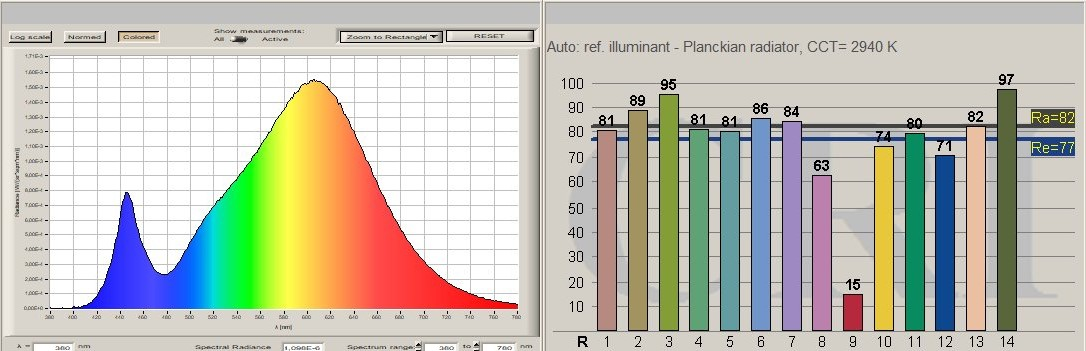
\includegraphics[width=1.0\textwidth]{bilder/cri2} 
% Bilddatei aus dem Unterverzeichnis bilder holen, skalieren auf 0.8*Satzspiegel
\caption {Messung einer warmweißen LED-Leuchte (Ausschnitt aus dem Demofile des Programmes \glqq LiVal\grqq von der Firma JETI): Links ist das Lichtspektrum der Leuchte dargestellt, rechts die gemessenen CRI-Werte  \protect\footnotemark}\label{b_cri2}
\end{figure}

 

 Daher ist auch mit einem einzigen Rot- und Hautton der CRI zu wenig ausschlaggebend, um damit eine Leuchte für Personenbeleuchtung zu bewerten (Kap. \ref{sec_auge}). Zusätzlich entsteht bei LED-Leuchtmitteln ein ähnliches Problem, wie bei den Leuchstoffröhren. Man kann das Spektrum mit den Peaks gut auf die Referenzfarben ausrichten, ohne das Gesamte Spektrum abdecken zu müssen. Gerade bei LED-Leuchten kann dieses Verhalten des CRI ausgenutzt werden, um kritische Bereiche zu verschleiern. Zusätzlich wird dies durch die arithmetische Mittlung der Referenzfarbwerte begünstigt. Ein, zwei schlechtere Werte mindern den $R_{a}$-Wert nicht beträchtlich. Beispielsweise wird bei Weißen-LEDs der fehlende Rotanteil nur am niedrigen $R_{9}$-Wert sichtbar, aber im CRI-Wert sind diese Schwächen einer LED-Leuchte kaum erkennbar \footnote{\cite{davis_ohno}}. Der CRI kann daher eher als richtungsweisend betrachtet werden: Eine Leuchte mit guter Farbwiedergabe wird auch immer einen guten CRI-Wert haben. Zum Vergleich für Leuchten eignen sich andere Farbwiedergabewerte heutzutage besser \footnote{\cite{production partner}}.\\\\
Aus diesen Gründen und der Erkenntnis der CIE, \emph{\glqq dass die CRI-Methode generell nicht anwendbar ist, um eine Anzahl von Lichtquellen gemäß ihrer Farbwiedergabe einzuordnen, wenn weiße LEDs darunter sind\grqq}\footnote{\citep[VI]{CIE}}, wird sich diese Arbeit hauptsächlich auf andere Farbwiedergabewerte konzentrieren, den CRI aber mit aufführen, weil dieser in der Scheinwerfer- und Fernsehbranche (noch) einen hohen Stellenwert inne hat.

\section{NIST: Color Quality Scale (CQS)} \label{sec_cqs}

Der Color Quality Scale, der von dem National Institute of Standards and Technology (NIST) erarbeitet wurde, orientiert sich an der Grundidee des CRI und versucht dessen Probleme anzugehen und ihn zu ersetzen. So gibt es fünfzehn voll saturierte Referenzfarben, die auch auf LED-Leuchten anwendbar sind. Über Skaleneffekte soll der CQS auch indirekt eine Aussage über die Farbwiedergabe von Pastelltönen ermöglichen (Abb. \ref{b_cqs1}). 

\begin{figure}[htp]     % h=here, t=top, b=bottom, p=page
\centering

\includegraphics[width=0.8\textwidth]{bilder/cqs} 
% Bilddatei aus dem Unterverzeichnis bilder holen, skalieren auf 0.8*Satzspiegel
\caption {Alle Referenzfarben des CQS mit voller Sättigung\protect\footnotemark}\label{b_cqs1}
\end{figure}

\footnotetext{\url{https://www.lemoledlight.com/wp-content/uploads/2016/04/LED-Lighting-CRI-5.jpg}}
Bei dem Farbvergleich des CRI wurden weniger Punkte für eine Farbe vergeben, wenn diese übersättigt wurde, also die Leuchte eine höhere Farbigkeit hatte als das Referenzlicht des CRI. Wenn beispielsweise eine Oberfläche eines Objekts beleuchtet wird, kann eine übersättigte Farbe jedoch hilfreich sein und ist daher nicht pauschal negativ einzuordnen. Deswegen wertet der CQS eine Übersättigung der Farbe nicht, nur eine Abweichung von Farbton oder Helligkeit wird bestraft. Außerdem errechnet sich der CQS aus dem quadratischen Mittel (root-means-square) der einzelnen Farben und es ist deutlicher erkennbarer, wenn einzelne Farbe schlechte Werte erzielen (Gleichung \ref{gl_cqs1})\footnote{\cite{davis_ohno}}.

\begin{equation}\label{gl_cqs1}
		\Delta E_{rms} = \sqrt{\frac{1}{15} \sum_{i=1}^{15} \Delta E_{i} ^{2}} 
\end{equation}

Aus diesem Farbdifferenzwert wird ähnlich wie beim CRI (Gleichung \ref{gl_cri1}) ein Farbwiedergabewerte errechnet (Gleichung \ref{gl_cqs2}).

\begin{equation}\label{gl_cqs2}
		Q_{f,rms} = 100 - 3,0305 \cdot \Delta E_{rms} 
\end{equation}

Schließlich wird der CQS auf Werte von 0 bis 100 skaliert. Dadurch entfallen beim CQS negative Farbwerte, die beim CRI sehr schwierig zu interpretieren sind (Gleichung \ref{gl_cqs3}). 

\begin{equation}\label{gl_cqs3}
		Q_{f} = 10 \ln(e^{\frac{Q_{f,rms}}{10}}+1) 
\end{equation}\\

Der CQS wird mit seinen fünfzehn Referenzfarborten (abhängig von der Farbtemperatur) im CIELAB-Farbraum eingezeichnet. Da die Abstände von Farborten in diesem Farbraum in etwa wahrgenommenen Farbunterschieden entsprechen (Kap. \ref{sec_lab}), kann man gut erkennen, wie stark sich die Farbwiedergabe einer Leuchte den Referenzwerten ähneln(Abb. \ref{b_cqs2a} und \ref{b_cqs2b}).\\

\begin{figure}[htp]     % h=here, t=top, b=bottom, p=page
\centering
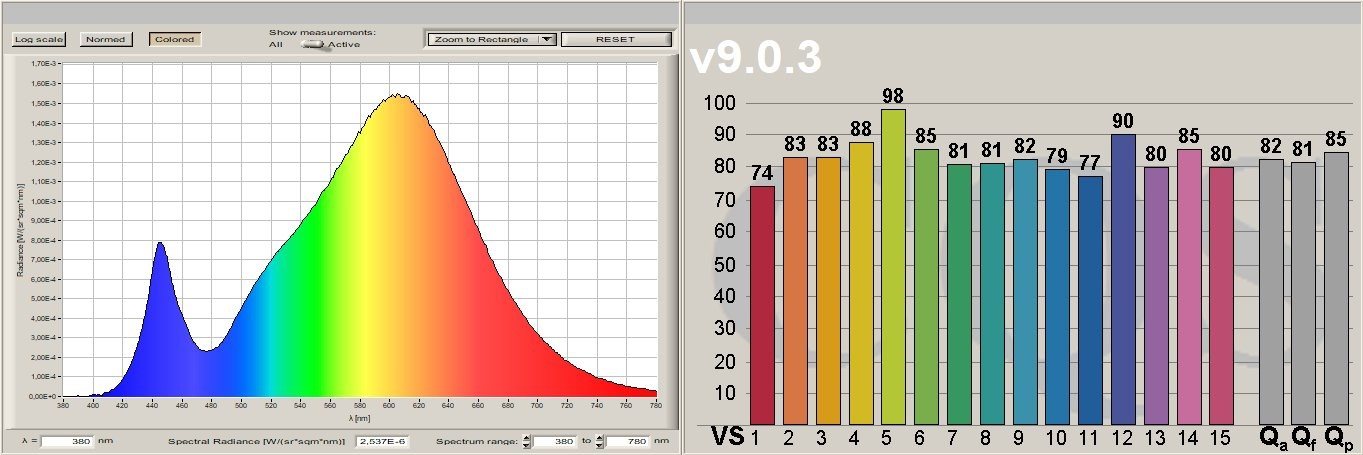
\includegraphics[width=0.9\textwidth]{bilder/cqs2a} 
% Bilddatei aus dem Unterverzeichnis bilder holen, skalieren auf 0.8*Satzspiegel
\caption {Ausschnitt aus dem Programm \glqq LiVal\grqq von der Firma JETI: Demo Spektrum einer warmweißen LED (2942K) mit $Q_{f} = 81$}\label{b_cqs2a}
\end{figure}

\begin{figure}[htp]     % h=here, t=top, b=bottom, p=page
\centering
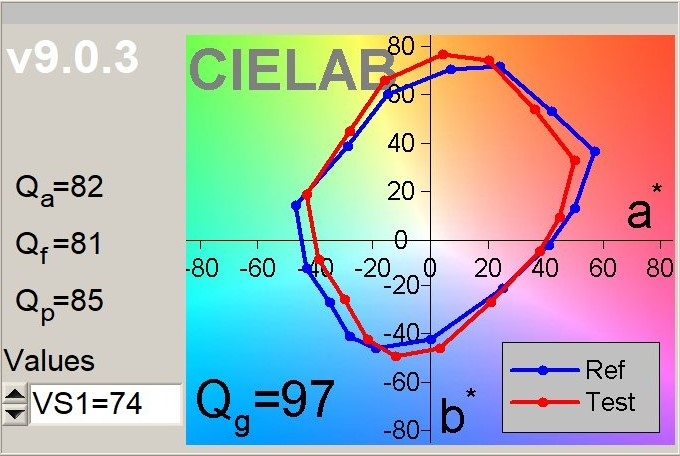
\includegraphics[width=0.7\textwidth]{bilder/cqs2b} 
% Bilddatei aus dem Unterverzeichnis bilder holen, skalieren auf 0.8*Satzspiegel
\caption {Ausschnitt aus dem Programm \glqq LiVal\grqq von der Firma JETI: Die fünfzehn Referenzfarben(blau) im CIELAB-Farbraum im Vergleich zu den gemessenen Werten (rot)}\label{b_cqs2b}
\end{figure}

Auf die in den Abbildung \ref{b_cqs2a} und \ref{b_cqs2b} erwähnten Werte $Q_{a}$ (optimierter CQS-Wert für kaum übersättigte Farben), $Q_{p}$ (optimierter CQS-Wert für viele übersättigte Farben) und $Q_{g}$(optimierter CQS-Wert im Zusammenhang mit dem Gamut Area Index) wird in dieser Arbeit nicht weiter eingegangen, weil sie über den Rahmen dieser Bachelorarbeit hinaus gehen\footnote{\cite[60-62]{khanh}}. \\
Da der CQS ähnlich wenige Referenzfarben nutzt wie der CRI, und keine besondere Aussage über die Farbwiedergabe von Hauttönen im TV-Bereich liefert, wird bei den Messungen dieser Arbeit das Hauptaugenmerk nicht auf dem CQS liegen. Der CQS eignet sich besser zur Einschätzung der Farbwiedergabe ohne Bezug zu einer TV-Kamera. 


\newpage 
\section{EBU: Television Lighting Consistency Index (TLCI)} \label{sec_tlci}
Der CRI-Wert einer Leuchte ist im Fernsehbereich kaum aussagekräftig, weil kein Bezug zur Videokamera besteht und die Farbwiedergabe von menschlichen Hauttöne kaum gemessen wird. Daher hat die European Broadcast Union (EBU) 2012 einen neuen Farbewiedergabe bestimmt, der auf den Film- und Fernsehbereich zugeschnitten ist, den Television Lighting Consistency Index.  
Wie eine Messung des TLCI vonstattengeht ist in diesem Blockschaltbild der EBU verdeutlicht (\ref{b_tlci1}):

\begin{figure}[htp]     % h=here, t=top, b=bottom, p=page
\centering
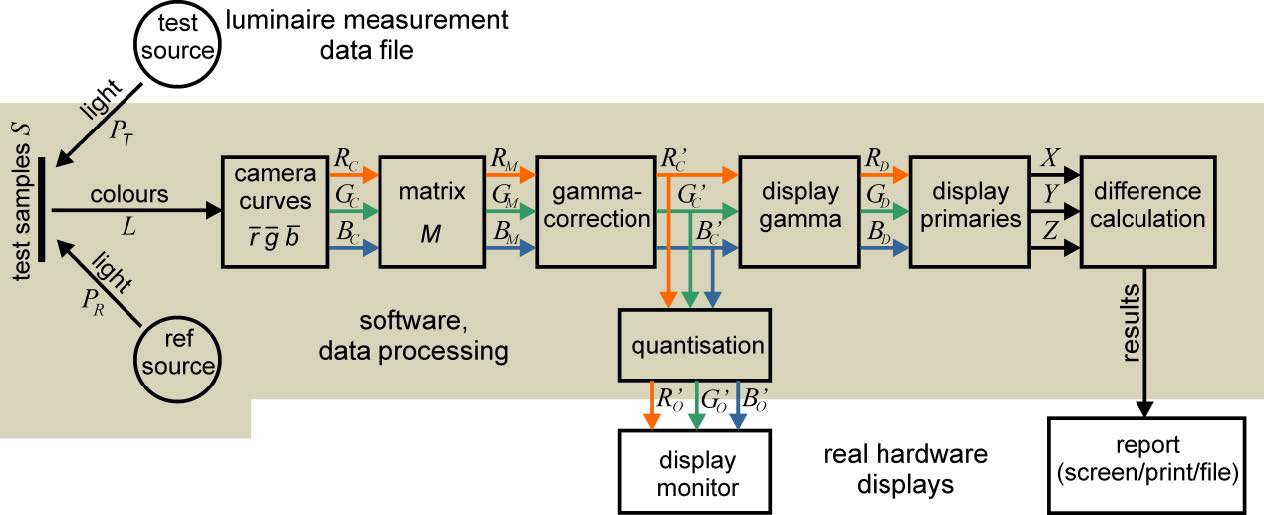
\includegraphics[width=1.0\textwidth]{bilder/tlci1} 
% Bilddatei aus dem Unterverzeichnis bilder holen, skalieren auf 0.8*Satzspiegel
\caption {Blockschaltbild einer TLCI-Wertbestimmung \protect\footnotemark}\label{b_tlci1}
\end{figure}
\footnotetext{\citep[15]{roberts}}
Die von der Kamera gefilmten Farben werden dann in einem Datenfile gespeichert. Die Daten werden analysiert, um die Farbtemperatur zu bestimmen und so die Referenzdaten zu erstellen.

Zur Ermittlung des TLCI wird eine Testtafel mit 24 Farben von einer \glqq Standartkamera\grqq gefilmt. Diese Tafel wird von der zu testenden Leuchte bestrahlt. Die Kamera ist an einen \glqq Standartbildschirm\grqq angeschlossen, auf dem die TLCI-Merssergebnisse angezeigt werden.
Im ersten Schritt gewichtet die Kamera die reflektierten Farben mit ihren $\bar{r}$-, $\bar{g}$- und $\bar{b}$-Kamerakurven und die Farbtemperatur wird bestimmt. Die so entstandenen $R_{C}$, $G_{C}$ und $B_{C}$-Werte werden dann im zweiten Schritt farblich abgeglichen ($R_{Cb}$, $G_{Cb}$ und $B_{Cb}$) und mit einer linearen Matrix M bewertet, um die Werte des RGB-Signals zu erhalten .
\begin{equation}\label{gl_tlci1}
\begin{bmatrix} R \\ G \\ B \end{bmatrix}= 
\begin{bmatrix} 1,182 & -0,209 & 0,027 \\ 0,107 & 0,890 & 0,003 \\ 0,004 & -0,134 & 1,094 \end{bmatrix}
\begin{bmatrix} R_{Cb} \\ G_{Cb} \\ B_{Cb} \end{bmatrix}
\end{equation}\\
Ein Weißabgleich wird vorgenommen und die RGB-Werte werden in einer zweiten Matrix verrechnet, damit die Sättigungswerte der Farben stimmen (Empfehlung der EBU: 90 \% Sättigung). Im nächsten Schritt werden die $R_{M}$, $G_{M}$ und $B_{M}$-Werte der einzelnen Farben von der Gammakurve der Kamera vorverzerrt.
Beim Bildschirm angekommen werden die R'G'B'-Werte der Farben mit der Gammakurve des Bildschirm wieder entzerrt (Empfehlung der EBU: $\gamma$ = 2,4). Für die 24 Farben werden dann im vorletzten Schritt mit der XYZ()-Matrix  die Farbkoordinaten X,Y und Z für den Bildschirm errechnet. Schließlich wird mit den Referenzenfarbwerten der selben Farbtemperatur die Farbunterschiede ermittelt (Gleichung \ref{gl_tlci1}).
\begin{equation}\label{gl_tlci1}
		\Delta E_{a} ^{*} = \left( {\sum_{i=1}^{18}(\Delta E_{i} ^{*})^{4}}  \right)^{\frac{1}{4}} 
\end{equation}
Das Ergebnis wird als TLCI-Wert ausgegeben. Für optimale Werte wird mit $k = 3,16$ (eine Tageslichtleuchtstoffröhre erreicht dabei den TLCI-Wert 50) und $p = 4$ (für ein balanciertes Verhältnis zwischen hohen und niedrigen Werten) gerechnet\footnote{\cite[16-22]{roberts}} (Gleichung \ref{gl_tlci2}).

\begin{equation}\label{gl_tlci2}
		Q = \frac{100}{1+(\frac{\Delta E^{*}}{k})^{p}}
\end{equation}

Der TLCI lässt wie der CQS keine negativen Ergebnisse zu (Kapitel \ref{sec_cqs}) und die Werte von 0-100 sind für den Coloristen in der Nachbearbeitung des Videomaterials wie folgt zu deuten(Tabelle \ref{t_tlci}):

	\begin{table}[htp] 
		\rowcolors{1}{}{lgray} 
		\centering
		\begin{tabular}{rlcc}  % Spalten nach Ausrichtung: l, c, r, p{breite} 
		\toprule
		\multicolumn{2}{c}{\large\sffamily Abstufungen des TLCI}\\ 							
		\midrule
		$100 \geq  Q_{a} \geq 85$  & Farben korrigierbar bzw. nicht notwendig\\ 
		$85 > Q_{a} \geq 75$ & nach Korrektur noch akzeptabel\\
		$75 > Q_{a} \geq 50$ & Aufbereitung sehr zeitaufwendig\\
		$50 > Q_{a} \geq 25$ & nicht mehr zu retten - verbesserbar\\
		$25 > Q_{a} \geq 0$ & ist und bleibt nicht akzeptierbar\\
		\bottomrule
		\end{tabular}
		\caption{$Q_{a}$ eingeteilt in verschiedene Stufen\protect\footnotemark}	
		\label{t_tlci}
	\end{table}
	\footnotetext{\cite{production partner}}
Anhand der Tabelle ist eine Art Kostenvergleich möglich, in dem die Farbwiedergabequalität einer Leuchte gegen den Nachbearbeitungsaufwand des Coloristen gegengerechnet werden kann. Der TLCI gibt sogar eine Empfehlung ab, an welchen Paramtern der Colorist Verbesserungen vornehmen muss (Abbildung \ref{b_tlci2}).\newpage 

Die Messung des TLCI-Werts ergibt ein Ergebnisprotokoll, bestehend aus drei Abschnitten: eine Farbtafel mit den 24 Farbfeldern, eine Empfehlung für den Coloristen zur nachträglichen Bildbearbeitung und ein Vergleich von Referenz- und Testspektrum (Abbildung \ref{b_tlci2}):\\ 

\begin{figure}[htp]     % h=here, t=top, b=bottom, p=page
\centering
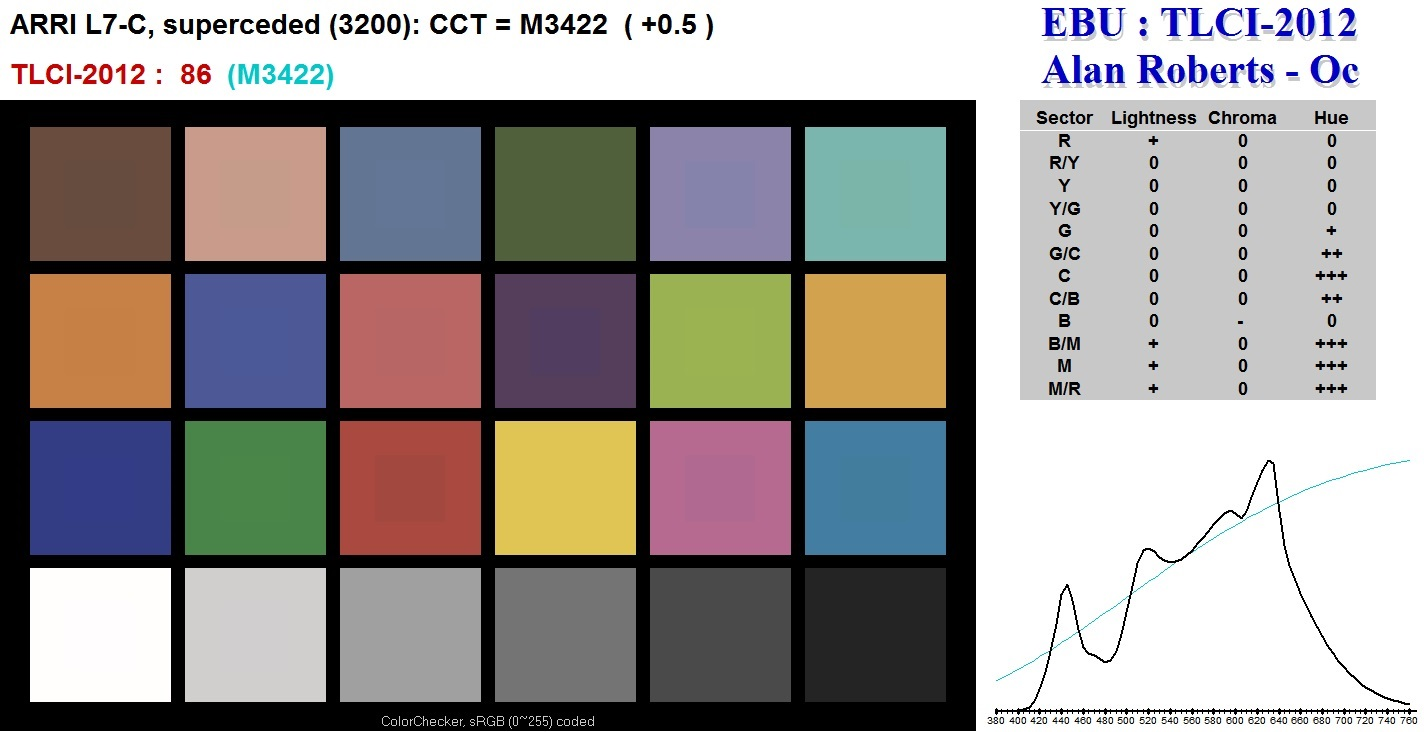
\includegraphics[width=1.0\textwidth]{bilder/tlci2} 
% Bilddatei aus dem Unterverzeichnis bilder holen, skalieren auf 0.8*Satzspiegel
\caption {TLCI-Ergebnisprotokoll eines Arri L7-C LED Fresnelscheinwerfers\protect\footnotemark}\label{b_tlci2}
\end{figure}
\footnotetext{\url{https://tech.ebu.ch/tlci-2012}}
Oben links ist der Name der Leuchte angegeben, die gemessene korrelierte Farbtemperatur (CCT) und die Abweichung vom Plank'schen Kurvenzug (\ref{sec_spektrum}) mit einer Gewichtung von 0.0054 (Empfehlung EBU). Ist der Abweichungswert kleiner als -1 wird die Zahl in magenta dargestellt (magentastichtiges weiß), ist sie größer als +1, in grün (grünstichiges weiß). Im Beispiel ist die Zahl daher schwarz. Eine Zeile darunter steht der gemessene TLCI-Wert. Der Arri L7-C ist mit $Q_{a}=86$ in die beste Farbwiedergabekategorie einzuordnen (Tabelle \ref{t_tlci}).\\
Oben rechts ist eine Tabelle mit Korrekturwerten für den Coloristen angegeben. Für 12 verschiedene Farbtöne wird jeweils ein Verbesserungsvorschlag für die Helligkeit, die Sättigung und die Farbtonabweichung angegeben. Da es nicht möglich ist, die Abweichung der Werte mit exakten Zahlen zu definieren, werden mit \glqq +\grqq, \glqq 0\grqq und \glqq -\grqq die verschiedenen Korrekturrichtungen aufgezeigt. Eine \glqq 0\grqq zeigt an, dass der Fehler zu klein ist, um ihn zu korrigieren. Die Anzahl der \glqq +\grqq und \glqq -\grqq wiederum ist ein Hinweis darauf, wie viel Aufwand der Colorist für die Anpassung benötigt. Der Arri L7-C hat beispielsweise Bedarf es vorallem im Bereich des Cyan, Blau/Magenta, Magenta und Magenta/Rot in der Farbtonabweichung einer Aufbesserung. Auch im Green/Cyan- und Cyan/Blau-Bereich sollte der Farbton angepasst werden. Die restlichen Verbesserungsvorschläge bei Helligkeit und Sättigung sollte der Colorist zügig bewältigen können.\\
Links unten ist eine Farbtafel mit den 24 Farben des TLCI sichtbar. Im großen Farbfeld ist die Farbe zusehen, wie das Licht des Arri L7-C diese Farbe wiedergibt. In der Mitte jeder Farbtafel ist ein kleineres Viereck, in dem die Referenzfarbe gezeigt wird. Je deutlicher also das Referenzviereck in dem Farbfeld zu sehen ist, desto schlechter ist die Farbwiedergabe der Testleuchte. Im Beispiel  ist im roten Farbfeld zu erkennen, dass der Arri L7-C diese Farbe nicht so gut wiedergibt wie andere Farben.\\ 
Rechts unten ist auf dem TLCI-Ergebnisprotokoll das Referenzspektrum von 380nm bis 740nm Wellenlänge abgebildet (schwarz) und dazu wird das geteste Spektrum geplotet (cyan). In dieser Ansicht kann man gut erkennen, inwieweit das Licht des Arri L7-C das Referenzspektrum abdeckt \footnote{\cite[15]{roberts}}.\\

Der TLCI sieht die Farben wie eine Kamera und zieht sogar zwei Hauttöne mit in Betracht. Daher eignet sich dieser Farbwiedergabewert sehr gut für die Messung der Auswirkung eines Red Tail.  



\section{IES Method for Evaluating Light Source Color Rendition (TM-30-15)} \label{sec_tm30}

Auch der TM-30 wurde 2015 von der \glqq Illuminating Engineering Society\grqq (IES) ausgearbeitet um eine Alternative zum CRI zu finden. Wie beim CRI werden ebenso bei der Messung des TM-30 Farbunterschiede zwischen einer Testleuchte und Referenzwerten der selben korrelierten Farbtemperatur aufgezeigt. Der TM-30 differenziert ähnlich, ob es sich bei der Testleuchte um einen Plank'schen Strahler  oder einem Tageslicht handelt. Zwischen einer CCT von 4500K und 5500K wird die Referenz proportional überblendet, um so zu verhindern, dass es bei 5000K einen \glqq Sprung\grqq gibt. Bei dem CRI konnte es nämlich passieren, dass eine Leuchte 2 unterschiedliche Referenzen bekam, je nach dem ob diese knapp über oder unter 5000K bei der Messung lag. 
Die 99 Referenzfarben (Color Evaluation Sample) wurden aus einem Pool von 105.000 Farbtönen realer Objekte statistisch ermittelt (Abbildung \ref{b_tm301}). Damit alle Farbtöne gleichmäßig abgedeckt werden, wurde der CAM02-UCS-Farbraum, der für seine Gleichmäßigkeit der Farbaufteilung bekannt ist, in Würfel eingeteilt. Von jedem dieser Würfel wurde dann eine der Referenzfarben bestimmt, die so gewählt ist, dass die unterschiedliche Wahrnehmung der verschiedener Wellenlänge minimal ist (Kapitel \ref{sec_auge}). Die große Anzahl der Referenzfarben verhindert, dass Leuchtenhersteller mit gezielten Peaks im Spektrum gute TM-30 Werte erreichen \footnote{\cite{usdep}}.
\newpage

\begin{figure}[H]     % h=here, t=top, b=bottom, p=page
\centering
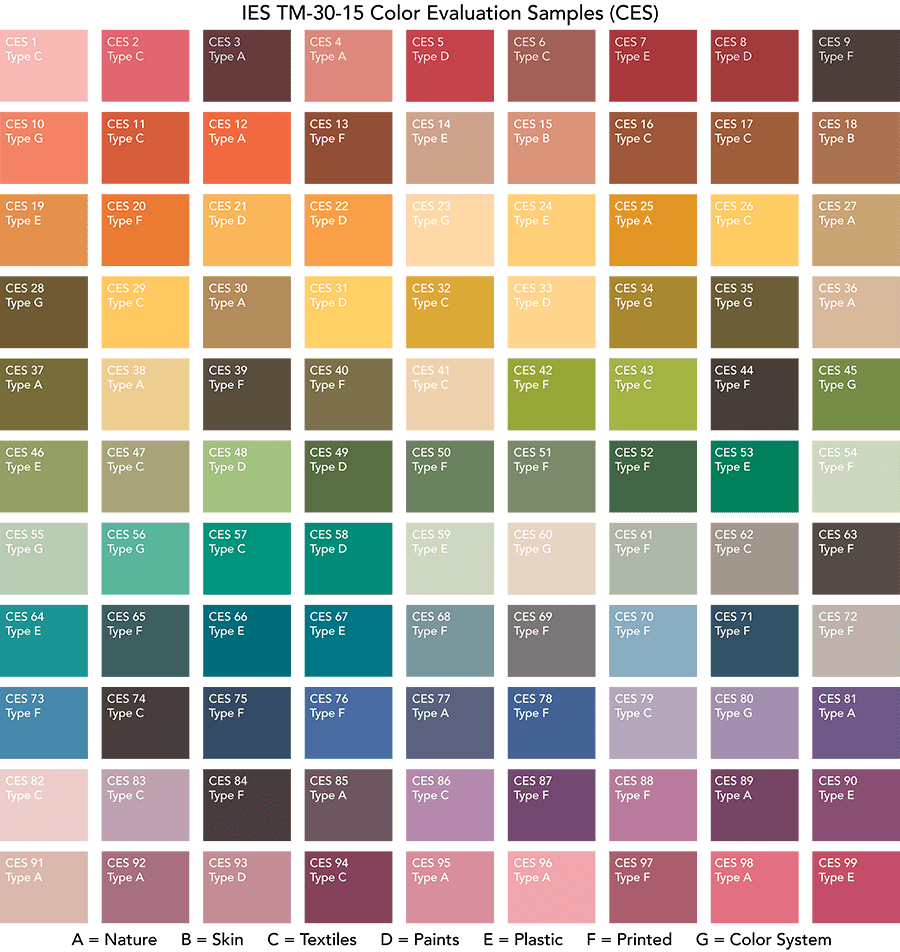
\includegraphics[width=1.0\textwidth]{bilder/tm301} 
% Bilddatei aus dem Unterverzeichnis bilder holen, skalieren auf 0.8*Satzspiegel
\caption {Alle 99 Referenzfarben des TM-30\protect\footnotemark}\label{b_tm301}
\end{figure}
\footnotetext{\url{https://agustos.com/wp-content/uploads/2017/10/TM30-color-samples-image.png}}


Im Gegensatz zum CRI spielen beim TM-30 zwei Werte eine große Rolle: $R_{f}$ und $R_{g}$. Der $R_{f}$-Wert bildet analog zum $R_{a}$-Wert des CRI ein Mittel aus den neunundneunzig Farbunterschieden denen einen Wert von 0 - 100 zugeordnet wird. Auch der $R_{f}$-Wert zeigt nicht an, ob die Leuchte übersättigte Farben hat oder einen Farbshift(\footnote{\cite[10]{royerhouser}}). Dazu wird der $R_{g}$-Wert gemessen. Dieser kann zwischen 60 und 140 variieren und zeigt so, ob die Farben übersättigt ($R_{g} > 100$), untersättigt ($R_{g} < 100$) sind oder mit dem Wert $R_{g} = 100$ genau die Farben der Referenzleuchte (bei selbiger Farbtemperatur) treffen. Mit dem $R_{f}$- und $R_{g}$-Wert wird ein X,Y-Koordinatensystem aufgespannt (Abbildung \ref{b_tm302}). Aus diesem Diagramm sind Farbwiedergabeeigenschaften einer Leuchte sehr gut ablesbar. Durch den zusätzlichen $R_{g}$-Wert gibt es nicht mehr nur Leuchten mit \glqq guter\grqq (hoher (hoher $R_{f}$)) oder \glqq schlechter\grqq (niedriger $R_{f}$) Farbwiedergabe. Zum Beispiel verliert eine Leuchte mit $R_{f}=82$ und $R_{g}=127$ gegenüber einer mit $R_{f}=90$ und $R_{g}=98$ nicht unweigerlich. Es kommt im direkten Vergleich viel mehr auf den Anwendungsfall an, in der die Leuchte gebraucht wird. Im sterilen Krankenhaus ist eine natürlich Farbwiedergabe wichtig, dort wäre die zweite Leuchte der Favorit, wohingegen für Superläden, in denen das Obst durch Übersättigung der Farben besser zur Geltung kommt, wäre die erste Lampe attraktiver. 
Daher ist der TM-30 viel flexibler zu deuten als der CRI, wo es immer nur um den höchsten $R_{a}$-Wert geht. Eine Möglichkeit könnte es sein, das X,Y-Koordinatensystem in verschiedene Bereiche(z.B. Fenster) einzuteilen, um so anwendungsspezifische Entscheidungen treffen zu können (\footnote{\cite[4]{royer}}).  


\begin{figure}[H]     % h=here, t=top, b=bottom, p=page
\centering
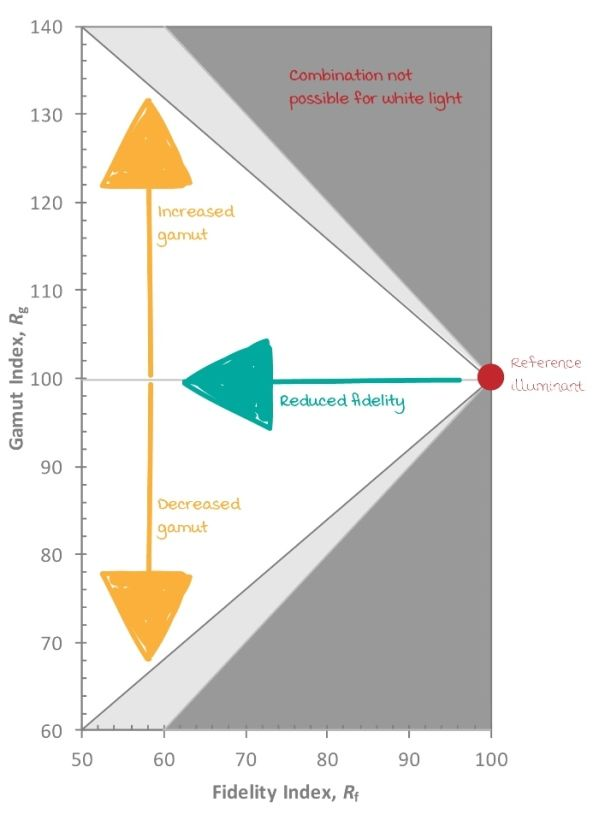
\includegraphics[width=0.5\textwidth]{bilder/tm302} 
% Bilddatei aus dem Unterverzeichnis bilder holen, skalieren auf 0.8*Satzspiegel
\caption {Koordinatensystem aus $R_{f}$ und $R_{g}$: Die hellgraue Zone steht für TM-30-Werte die nicht auf der Plank'schen Kurve liegen und die dunkelgraue Zone steht für alle Werte, die nicht mehr als \glqq weiß\grqq angesehen werden. \protect\footnotemark}\label{b_tm302}
\end{figure}
\footnotetext{\url{https://i.pinimg.com/originals/18/98/de/1898de3bdd8436fb5a1945d72a4c6772.jpg}}

In einer anderen Darstellung des $R_{g}$-Wert ist zu sehen, dass der Farbraum in 16 verschiedene \glqq binnings\grqq eingeteilt wurde. Jedes dieser \glqq binnings\grqq steht übergreifend für die in diesem Bereich liegende Farbtöne. In dieser Darstellung wird mit Pfeilen aufgezeigt, welche Anteile im Farbraum fehlen, welche übersättigt sind und welche den Farbton nicht treffen im Verhältnis zur Referenzfarbwiedergabe (Abbildung \ref{b_tm303}).

\begin{figure}[htp]     % h=here, t=top, b=bottom, p=page
\centering
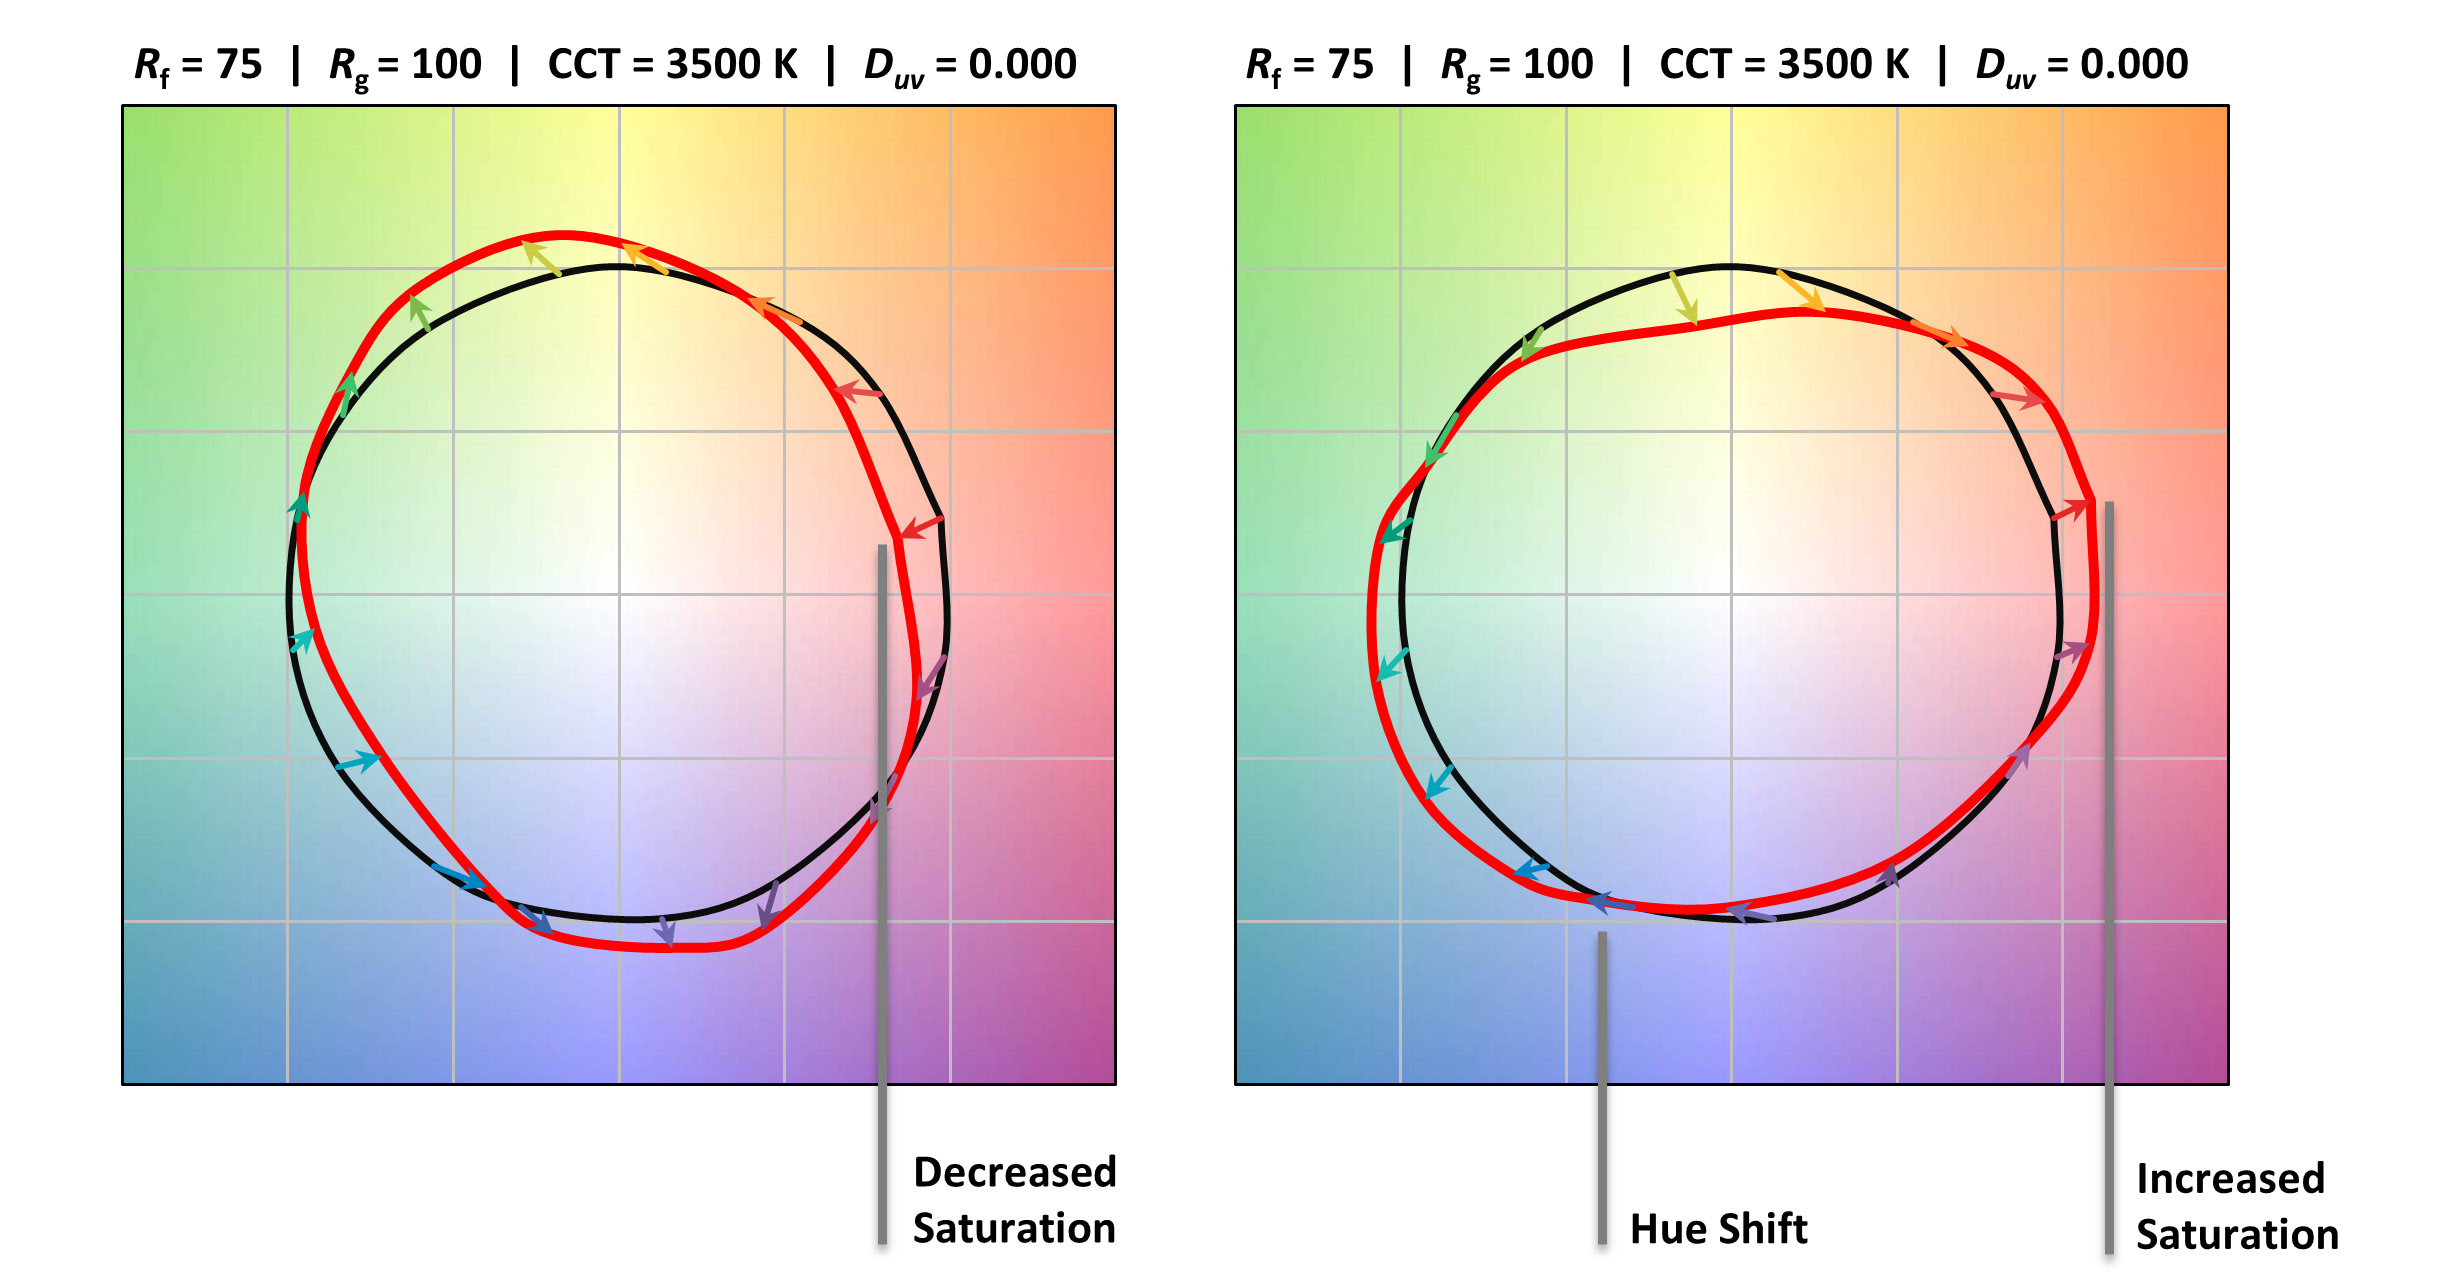
\includegraphics[width=1.0\textwidth]{bilder/tm303} 
% Bilddatei aus dem Unterverzeichnis bilder holen, skalieren auf 0.8*Satzspiegel
\caption {Wie sich die Farben der Testleuchte verhalten ist in der Vektorgraphik des $R_{g}$-Wertes anschaulich dargestellt. Der schwarze Kreis stellt die Referenzleuchte dar, der rote die getestete.  \protect\footnotemark}\label{b_tm303}
\end{figure}
\footnotetext{\cite{usdep}}

Bei der Messung einer Demo warmweiß LED gibt es viel an Messergebnissen zu protokollieren (Abbildung \ref{b_tm304}): Links oben wird gemessene $R_{f}$- und $R_{g}$-Wert angezeigt. Darunter ist die Vektorgraphik des $R_{g}$-Wertes dargestellt und darunter werden die $R_{f}$-Werte der 16 Farbraum-\glqq binnings\grqq  in einem Säulendiagramm präsentiert. In der Mitte ist der TM-30-Wert in seiner Koordinaten Darstellung aufzufinden und darunter werden die farblichen Abweichungen (in Prozenten) in einem Säulendiagramm dargestellt. Rechts oben wird analog zum TLCI das Spektrum der Leuchte im Verhältnis zum Referenzspektrum gezeigt und die gemessene korrelierte Farbtemperatur angegeben. Darunter gibt es eine Tabelle wo die farblichen Abweichung der einzelnen \glqq binnings\grqq als Zahlenwert angegeben werden. Schließlich findet man unter allem bisher genannten eine Säulendiagramm mit allen 99 Farben des TM-30. 
Das Ergebnis einer Messung ist mit diesen Daten nicht mehr schnell ersichtlich, wie beim CRI-Wert, hilft aber eine deutlich aussagekräftigere Entscheidung über eine Leuchte treffen zu können. 

\begin{figure}[H]     % h=here, t=top, b=bottom, p=page
\centering
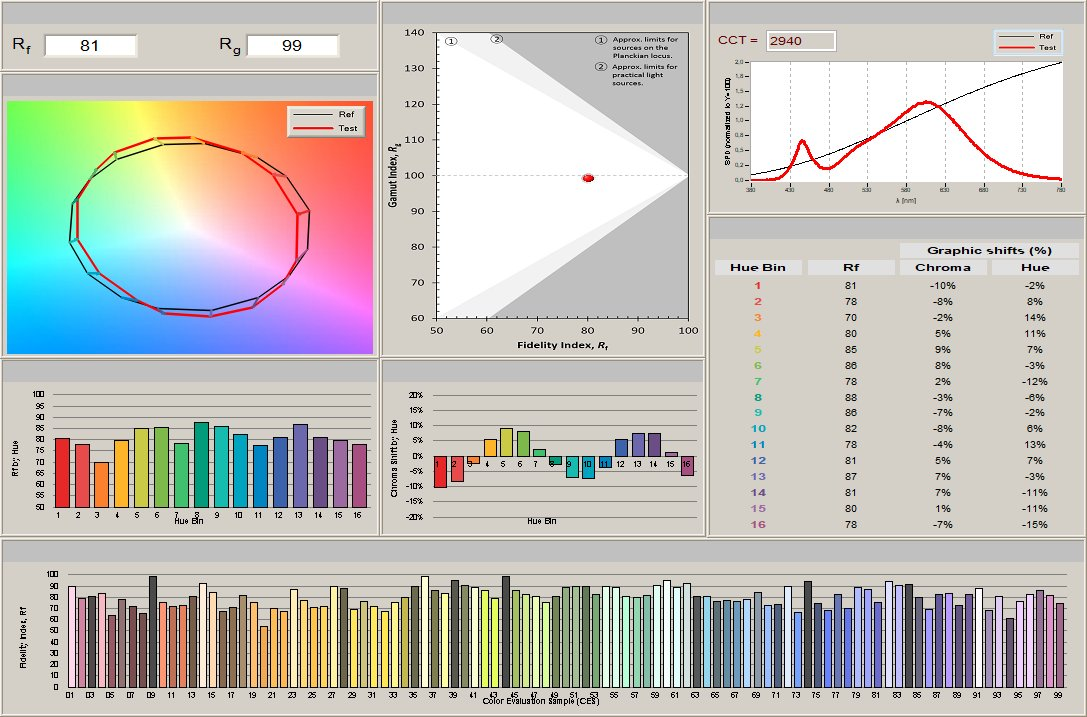
\includegraphics[width=1.0\textwidth]{bilder/tm304} 
% Bilddatei aus dem Unterverzeichnis bilder holen, skalieren auf 0.8*Satzspiegel
\caption {Wie sich die Farben der Testleuchte verhalten ist in der Vektorgraphik des $R_{g}$-Wertes anschaulich dargestellt. Der schwarze Kreis stellt die Referenzleuchte dar, der rote die getestete.  \protect\footnotemark}\label{b_tm304}
\end{figure}

Der TM-30 



\chapter{Leuchtmittel}

\section{Glühlampe} \label{sec_glühlampe}

\section{Halogenglühlampe} \label{sec_halogenglühlampe}

\section{Entladungslampen} \label{sec_entladungslampe}

\section{LEDs} \label{sec_led}

\chapter{Vormessungen}

\section{Ziel}

\section{Aufbau}

\section{Fazit aus der Vormessung}

\chapter{Hauptmessung}

\section{Messaufbau}

\chapter{Messergebnisse}

\section{Unterkapitel mit Mathematik, Bildern und Querverweisen}

\chapter{Umfrage}

\section{Unterkapitel mit Mathematik, Bildern und Querverweisen}

\chapter{Umfrageergebnisse}

\section{Unterkapitel mit Mathematik, Bildern und Querverweisen}

\chapter{Auswertung aller Ergebnisse}

\section{Unterkapitel mit Mathematik, Bildern und Querverweisen}

\chapter{Fazit}

\section{Unterkapitel mit Mathematik, Bildern und Querverweisen}





%--------------------- VERZEICHNISSE ----------------

\listoffigures % Abbildungsverzeichnis erzeugen
\listoftables % Tabellenverzeichnis erzeugen

%--------------------- LITERATURLISTE ---------------
% Die Einträge sollen alphabetisch sortiert sein.

\begin{thebibliography}{}

% Formatierung für Internetquelle
% Grundregel: Name, Vorname (falls vorhanden), VÖ-Jahr (falls vorhanden), Titel in Anführungszeichen, URL, Datum des letzten Aufrufs
% zur Formatierung der URL unbedingt den url-Befehl benutzen!!!

\bibitem[Bladowski \& Maus(2010)]{unimann}
Bladowski, Beate \& Maus, Daniel:
\emph{\glqq Farbwahrnehmung\grqq}
\url{http://irtel.uni-mannheim.de/lehre/seminararbeiten/w96/Farbe/seminar.htm#Wieviele}, 15.07.2010, letzter Zugriff 28.06.2018

\bibitem[Royer \& Houser(2015)]{royerhouser}
Royer, Micheal \& Houser Kevin:
\emph{\glqq Understanding and Applying TM-30-15\grqq}
\url{https://www.energy.gov/sites/prod/files/2015/09/f26/tm30-intro-webinar_9-15-15.pdf}, 15.09.2015, letzter Zugriff 26.06.2018

\bibitem[U.S. Department of Energy(2015)]{usdep}
U.S. Department of Energy:
\emph{\glqq Evaluating Color Rendition Using IES TM-30-15\grqq}
\url{https://www.energy.gov/sites/prod/files/2016/04/f30/tm-30_fact-sheet.pdf}, Oktober 2015, letzter Zugriff 25.06.2018

\bibitem[Commission Internationale de l'Eclairage(2007)]{CIE}
Commission Internationale de l'Eclairage:
\emph{\glqq Technical Report 177:2007 : Color Rendering of White LED Light Sources\grqq}
\url{https://de.scribd.com/document/125319182/CIE-177-2007}, 2007, letzter Zugriff 20.06.2018

\bibitem[Davis \& Ohno(2006)]{davis_ohno}
Davis, Wendy L. \& Ohno, Yoshihiro:
\emph{\glqq Development of a Color Quality Scale\grqq}
\url{http://citeseerx.ist.psu.edu/viewdoc/download?doi=10.1.1.568.8399&rep=rep1&type=pdf}, 08.02.2006, letzter Zugriff 20.06.2018

\bibitem[DocCheck Flexikon(2014)]{doccheck sko}
DocCheck Flexikon:
\emph{\glqq Skotopisches Sehen\grqq}
\url{http://flexikon.doccheck.com/de/Skotopisches_Sehen}, 24.01.2014, letzter Zugriff 18.06.2018

\bibitem[DocCheck Flexikon(2014)]{doccheck pho}
DocCheck Flexikon:
\emph{\glqq Photopisches Sehen\grqq}
\url{http://flexikon.doccheck.com/de/Photopisches_Sehen}, 10.05.2016, letzter Zugriff 18.06.2018

\bibitem[Production Partner(2018)]{production partner}
Production Partner:
\emph{\glqq Farbwiedergabe: TM-30-15, CRI und Co.\grqq}
\url{https://www.production-partner.de/basics/farbwiedergabe-tm-30-15-cri-und-co/}, 22.02.2018, letzter Zugriff 20.06.2018


\bibitem[Gigahertz-Optik(2012)]{Gigahertz}
Gigahertz-Optik:
\emph{\glqq Grundladen der Lichtmesstechnik\grqq}
\url{https://www.gigahertz-optik.de/de-de/grundlagen-lichtmesstechnik/}, letzter Zugriff 20.06.2018


% Formatierung für Aufsatz / Paper: Titel in Anführungszeichen, Zeitschriftentitel kursiv

\bibitem[Royer(2016)]{royer} 
Royer, Michael P.:
\glqq IES TM-30-15 Is Approved—Now What?\grqq, 
\emph{LEUKOS} vol. 12 (1-2, 3-5), 2016


\bibitem[Dooley \& Streicher(1982)]{dooley_streicher} 
Dooley, Wesley L.  \& Streicher, Ronald D.:
\glqq M--S Stereo: A Powerful Technique for Working in Stereo\grqq, 
\emph{Journ. Audio Engineering Society} vol. 30 (10), 1982

% Formatierung für Fachbuch, Diplomarbeit o.Ä.: Titel kursiv
\bibitem[Roberts(2015)]{roberts}
Roberts, Alan: 
\emph{TELEVISION LIGHTING CONSISTENCY INDEX (TLCI-2012)}, Version 2.015e, 18.04.2015

\bibitem[Hentschel(1993)]{hentschel}
Hentschel, Hans-Jürgen: 
\emph{Licht und Beleuchtung Theorie und Praxis der Lichttechnik}, 4. Aufl., Hüthig 1994

% Formatierung für Fachbuch mit Herausgeber und mehreren Autoren
\bibitem[Spehr(2009)]{spehr}
Spehr, Georg (Hrsg.): 
\emph{Funktionale Klänge}, transcript 2009

\bibitem[Greule(2014)]{greule}
Greule, Roland (Autor):
\emph{Licht und Beleuchtung im Medienbereich}, Hanser 2015 

\bibitem[Khanh \& Bodrogi \& Vinh(2007)]{khanh}
Khanh, Tran Quoc (Autor) \& Bodrogi, Peter (Autor) \& Vinh, Trinh Quang (Autor):
\emph{Color Quality of Semiconductor and Conventional Light Sources}, Wiley-VCH 2017


% Formatierung für ein einzelnes Kapitel eines speziellen Autors aus einem Fachbuch mit mehreren Autoren
\bibitem[Sowodniok(2009)]{sowodniok}
Sowodniok, Ulrike: 
\glqq Funktionaler Stimmklang -- Ein Prozess mit Nachhalligkeit\grqq, 
in: Spehr, Georg (Hrsg.): \emph{Funktionale Klänge}, transcript 2009




% Formatierung für Aufsatz / Paper: Titel in Anführungszeichen, Zeitschriftentitel kursiv
\bibitem[Stephenson(1990)]{stephenson}
Stephenson, Uwe: 
\glqq Comparison of the Mirror Image Source Method and the Sound Particle Simulation Method\grqq, 
\emph{Applied Acoustics} vol. 29, 1990


\end{thebibliography}

%--------------------- EIGENSTÄNDIGKEITSERKLÄRUNG ---------------
\clearpage\thispagestyle{empty}
\eigen  % im header definiert
%--------------------------------------- ENDE ------------------------------------
\end{document}
%%%%%%%%%%%%%%%%%%%%%%%%%%%%%%%%%%%%











